\documentclass[11pt]{extarticle}
\usepackage{manualdoprofessor}
\usepackage{fichatecnica}
\usepackage{lipsum,media9}
\usepackage[justification=raggedright]{caption}
\usepackage[one]{bncc}
\usepackage[lunna]{../edlab}
\usepackage{marginnote}
\usepackage{pdfpages}
\usepackage[printwatermark]{xwatermark}
\newwatermark[pagex=2]{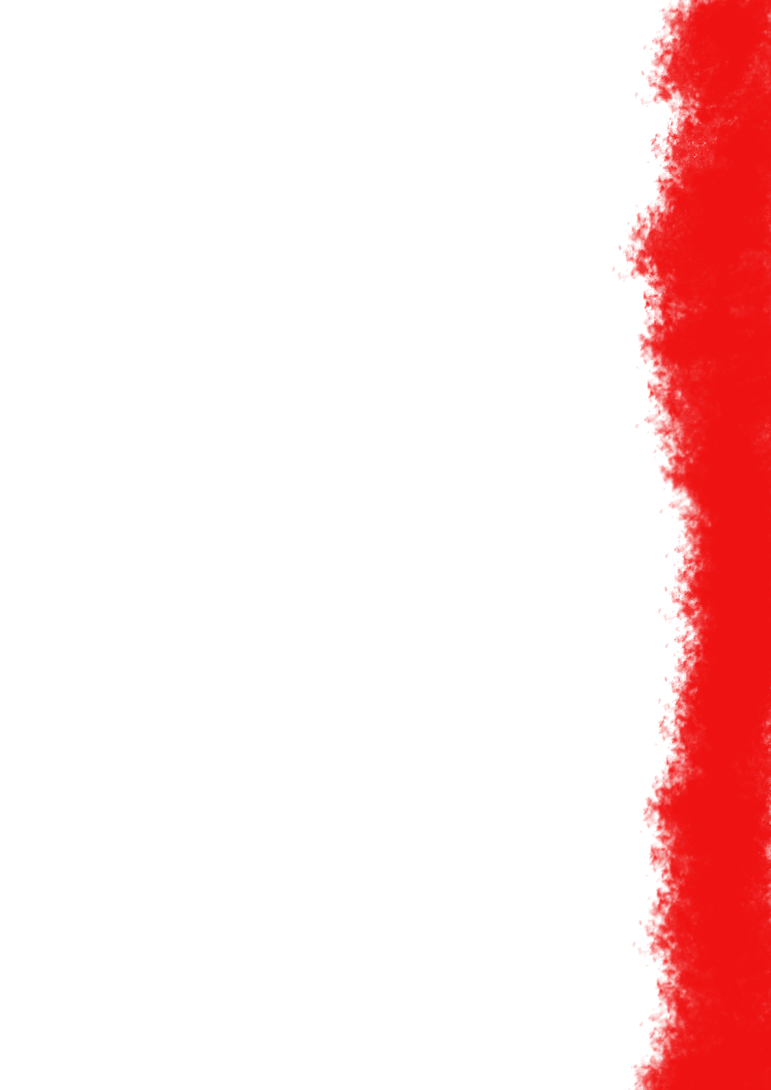
\includegraphics[scale=3.3]{watermarks/test-a.png}}	% página específica
%\newwatermark[oddpages]{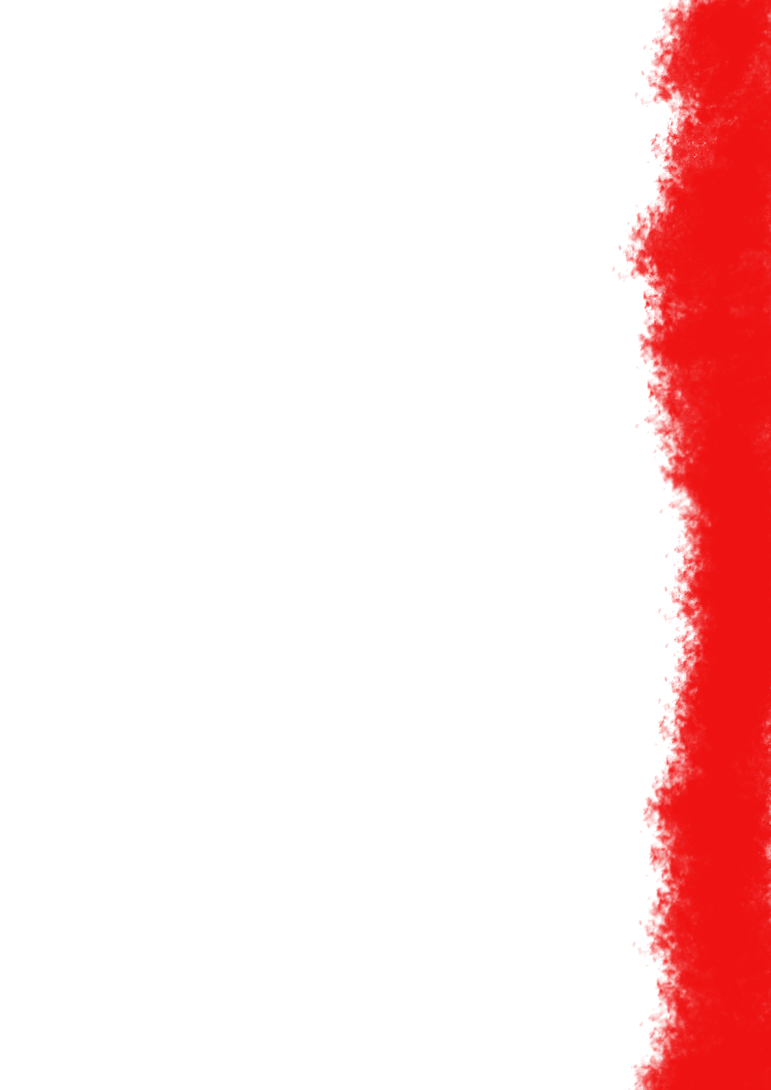
\includegraphics{watermarks/test-a.png}}			% páginas ímpars
%\newwatermark[evenpages]{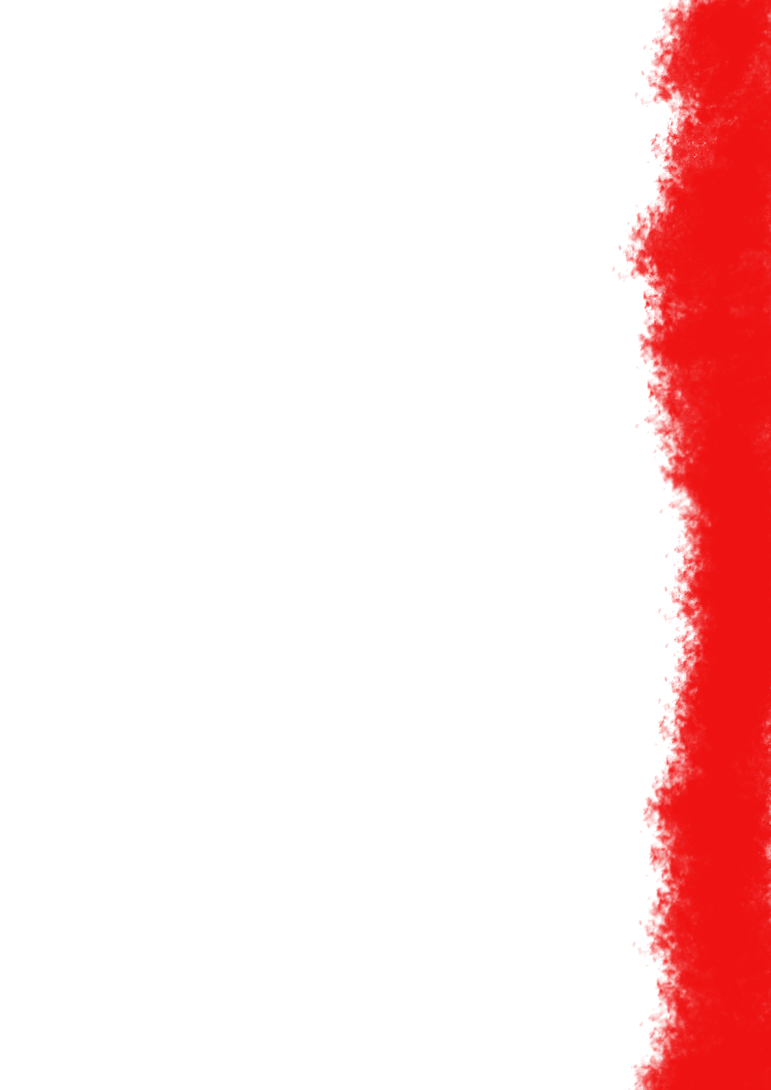
\includegraphics{watermarks/test-a.png}}			% págimas pares
\newwatermark[allpages]{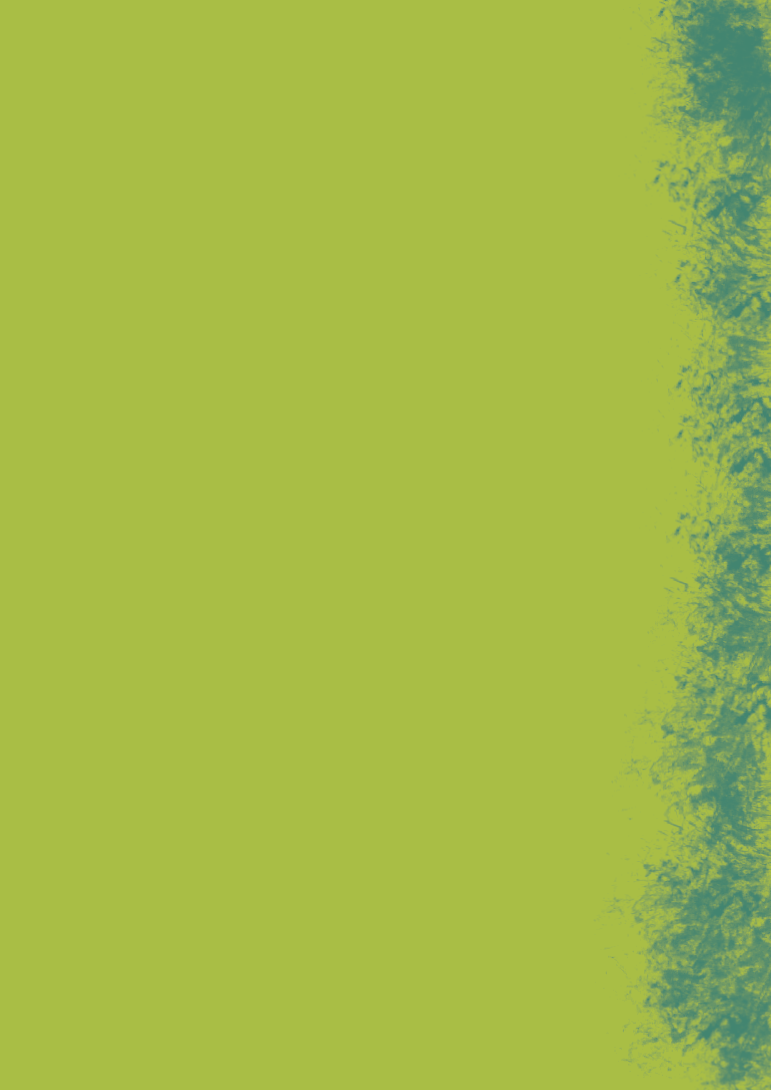
\includegraphics[scale=3.3]{watermarks/test-b.png}}

\pagecolor{cyan!0!magenta!10!yellow!28!black!28!}

\newcommand{\AutorLivro}{Aline Abreu}
\newcommand{\TituloLivro}{Banguela}
\newcommand{\Tema}{Quotidiano de crianças nas escolas; nas famílias e nas comunidades (urbanas e rurais)}
\newcommand{\Genero}{Narrativos: fábulas originais; da literatura universal e da tradição popular; etc}
%\newcommand{\imagemCapa}{./images/PNLD0001-01.png}
\newcommand{\issnppub}{978-65-99448-45-4}
\newcommand{\issnepub}{978-65-99448-47-8}
% \newcommand{\fichacatalografica}{PNLD0001-00.png}
\newcommand{\colaborador}{{Paulo Pompermaier e Renier Silva}}

\begin{document}

\title{\TituloLivro}
\author{\AutorLivro}
\def\authornotes{\colaborador}

\date{}
\maketitle

%\begin{abstract}\addcontentsline{toc}{section}{Carta ao professor}
%\pagebreak

\tableofcontents



\section{Sobre o livro}

%27 caracteres
\paragraph{O livro} 
``Banguela'' narra a ansiedade de um menino para que seu dente caia e ele fique banguela como os seus colegas.

%822 caracteres
\paragraph{Descrição} 
Com ilustrações que acompanham e complementam a narrativa verbal, a queda do dente
da frente é esperada pelo menino como um grande evento festivo. Desde a capa, vemos a imagem
de um balanço de brincar, que se repete no decorrer das páginas. O mundo ao redor do menino
mimetiza seu desejo interno e tudo remete ao tão esperado evento. 
O fato de na escola haver muitos colegas que já são banguelas instiga sua imaginação.
A queda do dente será divertida como brincar num balanço. E o é, mas não só para a personagem,
como também para o pequeno leitor, já que este momento da narrativa é construído por meio 
de uma ação performática: o dente, que estava por um fim, cai devido à força com que a
criança leitora virou a página, segundo o menino do livro. Por fim, na comemoração por enfim
ter se tornado banguela, mais um dente cai, para maior surpresa e diversão. 

%411 caracteres
\paragraph{Competências} 
São muitas as competências que este livro trabalha com as crianças
da \textbf{Pré-escola}. A começar pela estrutura narrativa verbal e não verbal
que apresenta o livro. A capacidade de ouvir uma história sendo narrada é essencial no 
desenvolvimento humano, e é prescritivo para o seguinte passo de narrar as próprias
histórias bem como aquelas que ouviu. Esta introdução ao mundo narrativo não se dá
somente por meio das palavras, mas também pelas imagens, que são outra forma de 
representar o mundo. Igualmente, as crianças aprendem a ler as imagens e, então, 
contar histórias a partir de imagens criadas por elas mesmas. 
NO que se refere ao conteúdo da narrativa, o livro serve apra amenizar um assunto
que pode causar ansiedade negativa em algumas crianças. Há os que, como a personagem,
anseiam positivamente por este momento, mas há também aqueles que o temem. 
Para estes últimos, a história pode servir como inspiração para transformar em 
diversão e prazer o ato de perder um dente e virar banguela. 
Afinal é esta uma das funções das narrativas na vida humana: dar sentido aos 
fenômenos naturais, como a queda de um dente, na infância, e assuntos mais complexos
no decorrer do tempo. Por isso, este livro é uma ótima forma de introduzir os pequenos
leitores neste mundo da literatura. 


%862 caracteres
\paragraph{Aprofundamento} 
Este material tem a intenção de contribuir para que você consiga desenvolver um trabalho aprofundado 
com esta obra na sala de aula. Você encontrará informações sobre o autor, sobre 
o gênero e sobre os temas trabalhados ao longo do livro. Apresentaremos também 
algumas propostas de trabalho para a sala de aula que você poderá explorar livremente, 
da forma que considerar mais apropriada para os seus estudantes. Para a prática 
da Literacia Familiar, oferecemos um guia que pode ajudar nas orientações aos 
responsáveis pela criança, para incentivar o gosto pela leitura e contribuir para 
que os estudantes desenvolvam em casa habilidades que serão importantes no momento 
da alfabetização. Por fim, você encontrará sugestões de livros, artigos e sites 
selecionados para enriquecer a sua experiência de leitura e, 
consequentemente, a de seus estudantes.


\section{Sobre o autor}

%532 caracteres
\paragraph{A autora} 
Aline Abreu nasceu em Barra do Piraí, no Rio de Janeiro. Ministra oficinas de artes e cursos teóricos e práticos para crianças e adultos. É também professora do curso de graduação em Artes Visuais da Faculdade Santa Marcelina/\textsc{sp}.

%313 caracteres
\paragraph{Publicações} 
É também autora de outros oito livros, entre eles, ``Mágica – Nina \& Ludovico'' (2020), ``Este não é o presente que eu pedi'' (2015), ``Menina amarrotada'' (2013), ``Cheirinho de talco'' (2012) e ``Cada família é de um jeito'' (2006).

%358 caracteres
\paragraph{Currículo} 
A autora é formada em Artes Visuais pela \textsc{faap/sp} e mestre em Crítica Literária pela \textsc{puc/sp}. 
Em 2016, ganhou o Prêmio João de Barro de livro ilustrado com o livro ``Quase ninguém viu'' (2019), livro que também foi agraciado com o selo Distinção Cátedra da Cátedra \textsc{unesco} de Leitura \textsc{puc/rj} em 2019. Em 2020, ganhou o troféu Monteiro Lobato de literatura infantil da revista Crescer.


\section{Sobre o gênero}

%55 caracteres
\paragraph{O gênero} O gênero deste livro é \textit{narrativa}. 

%596 caracteres
\paragraph{Descrição} 
O gênero narrativo possui uma variedade de tipos e, cada um, suas estruturas específicas.
A característica comum entre todos é que sempre há uma história a ser contada, com linearidade,
ou seja, começo, meio e fim, e personagens. 
Dentre os tipos de narrativas mais comuns na literatura infantil, estão: mito, lenda, 
fábula e apólogo. Este último, semelhante à fábula, possui personagens não humanos, 
dramatização de fala, e uma moral, implícita ou explícita, mas difere na natureza destas 
personagens: se no caso da fábula se trata de animais, no caso do apólogo as personagens 
são objetos inanimados. No caso deste livro, a pinta de uma joaninha, que é mais um 
símbolo do que um objeto. Quase qualquer coisa pode ser uma personagem de uma narrativa 
infantil, já que a capacidade reflexiva das crianças nesta idade ainda está em um nível primário. 


%603 caracteres
\paragraph{Interação} 
As narrativas são uma forma de inserir os sujeitos no mundo. 
São elas que apresentam boa parte dos valores culturais da sociedade 
onde se vive. Mas não é só passivo o papel das crianças nesta experiência. 
As interações entre dois ou mais personagens onde se verifica
uma ação de linguagem organiza e impulsiona experiências compartilhadas,
importantes para o desenvolvimento psíquico do sujeito nos primeiros anos de vida.
Neste sentido, as narrativas são uma ótima ferramenta para
apresentar o mundo e capacitar as crianças para viver nele, mas como se
trata de um trabalho com a linguagem, sempre dando espaço à individualidade, 
seja na compreensão das histórias, na identificação com as personagens, ou 
no ato de narrar. 

%862 caracteres
\paragraph{Competências} 
Para além da narrativa, o livro apresenta às crianças uma linguagem artística complexa.
Explorar as cores, as formas, o posicionamento das personagens 
na página e até mesmo a opinião e os sentimentos das crianças sobre as imagens 
são possibilidades que aprofundarão a leitura, aumentarão o repertório 
e incentivarão o desenvolvimento do vocabulário e da fluidez do discurso. 

\section{Temas}

\subsection{Quotidiano de crianças nas escolas; nas famílias e nas comunidades (urbanas e rurais)}

%136 caracteres
\paragraph{Abordagem} 
O livro aborda um fato do quotidiano de toda criança que é a queda dos dentes de leite.
%206 caracteres
\paragraph{Descrição} 
Um menino anseia pela queda de seu dente de leite para que, como seus colegas, ele fique banguela.
Este acontecimento é visto como uma grande promessa de diversão retratada no livro 
pela semelhança entre o balançar dos dentes e o movimento de um balanço num
parque de diversões.
%275 caracteres
\paragraph{Competências} 
Este tema se relaciona sobretudo ao campo de experiência ``Corpo, gestos e movimentos'', descrito pela
\textsc{bncc}, que tem como intuito trabalhar o corpo como instrumento expressivo e comunicativo por excelência, 
que serve de suporte para o desenvolvimento emocional e mental, sendo essencial na construção de afetos e conhecimentos.

\section{Modelagem de aula}
A seguir você encontrará a descrição de uma aula modelo como exemplo 
prático de exploração do livro com estudantes. Esta seção apresentará 
orientações sobre como organizar a sala de aula para receber os 
estudantes, exercitar a interação verbal e prepará-los para o 
momento da leitura.

Em seguida, você encontrará a \textbf{Leitura dialogada}, um 
tópico destinado a te orientar para o momento específico da 
leitura com os estudantes. Por fim, no tópico 
\textbf{Propostas de atividades}, você encontrará ideias 
de práticas que pode explorar com as crianças em sala de 
aula após a leitura. 

Essas atividades podem ser trabalhadas de acordo com a 
disponibilidade do seu cronograma e fique à vontade para adaptá-las 
da forma que achar melhor para os seus estudantes. Cada turma é única 
e o seu conhecimento prático das características de cada aluno será 
essencial para definir a melhor forma de aplicar essas ideias. 

O objetivo deste manual é oferecer algumas ideias 
e inspirações para um trabalho que pode ser desenvolvido tanto 
a curto, quanto a médio e longo prazo. Sinta-se a vontade para 
personalizar a aula e torna-la sua, aplicando seus conhecimentos, sua 
personalidade e aproveite para fortalecer 
seu vínculo com a turma.


\subsection{Antes de ler}

\BNCC{EI03EO06} 
\BNCC{EI03EF03} 
\BNCC{EI03EF04} 
\BNCC{EI03EF06} 
\BNCC{EI03EF07} 
\BNCC{EI03EF08} 
\BNCC{EI03EF09}

%Alterar o nível escolar nesse parágrafo.
Como este trabalho será realizado com crianças da \textbf{Pré-escola}, 
que ainda não têm muita intimidade com o livro enquanto objeto, você terá o 
papel de mediar este contato. 

Nosso objetivo é que os próprios estudantes possam manusear 
e explorar o livro de forma autônoma, mas, para que isto aconteça, você 
pode ajudar a tornar o caminho mais convidativo com atividades que tenham 
intencionalidade educativa. 

A \textsc{bncc} define intencionalidade educativa como ``organização 
e proposição, pelo educador, de experiências que permitam às crianças 
conhecer a si e ao outro e de conhecer e compreender as relações com a 
natureza, com a cultura e com a produção científica, que se traduzem nas 
práticas de cuidados pessoais (alimentar-se, vestir-se, higienizar-se), 
nas brincadeiras, nas experimentações com materiais 
variados, na aproximação com a literatura e no encontro com as 
pessoas''.\footnote{\textsc{bncc}, página 39}

É importante manter essa intencionalidade em mente não apenas na condução 
das atividades propostas neste manual, mas também para aproveitar as 
oportunidades espontâneas de construir conhecimentos que podem surgir durante 
a interação direta com os estudantes.

\begin{enumerate}
%836 caracteres
\item \textbf{O ambiente}\quad Antes de iniciar o trabalho com o livro, é importante que você 
prepare o ambiente para receber a turma. Como o trabalho com o livro terá 
três momentos (antes, durante e depois da leitura), seria interessante que você 
criasse um ambiente para cada etapa. Nas \textbf{Sugestões de referências complementares} 
você encontrará um artigo que discorre sobre a importância da organização da sala 
de aula para a educação infantil, que pode ser um bom guia para a criação desses 
ambientes. Para o momento antes da leitura, você pode dispor pela sala de aula
imagens animadas de dentes, pendurados, espalhados no chão, em lugares
mais escondidos\dots{} Você também pode, se possível, dispor pelúcias e fantoches, 
de dentes, fadas do dente\dots{}

%413 caracteres
\item \textbf{Primeira opção}\quad Utilize os primeiros 
momentos da aula para passear por essa área, introduzindo as crianças
neste universo. Deixe-os à vontade para brincar com os objetos,
numa caça aos dentes, por exemplo, ou imitando a voz da fada dos
dentes. São diversas as possibilidades de brincadeira com estes
objetos. O importante é que elas se familiarizem o assunto
que será tratado em seguida.
%632 caracteres
\item \textbf{Segunda opção}\quad 
Outra opção para este primeiro momento é, se possível, 
levar as crianças para a área externa da escola onde estão os brinquedos,
em especial o balanço. Todos devem se balançar ao menos um pouco. 
Estabeleça uma ordem: quem se balançou primeiro, agora vai 
empurrar o coleguinha. Alerte para a intensidade da força: não pode ser muito
para que o outro não caia nem se machuque, só o suficiente para balançar 
e se divertir.

\end{enumerate}


\subsubsection{A interação verbal} 
Criar situações em que as crianças precisam dialogar diretamente com 
você é uma das práticas mais importantes de Literacia, pois elas estimulam 
o desenvolvimento linguístico, ampliam o vocabulário e reforçam a 
capacidade dos estudantes de compreenderem o que ouvem e se expressarem 
pela fala. O diálogo livre com a criança também reforça sua autoestima, pois 
a faz se sentir ouvida e valorizada pelo adulto, ao vê-lo prestar atenção 
no que ela tem a dizer. Portanto, sempre que possível, reserve um tempo na 
aula apenas para a interação verbal. 

Como esse tipo de interação é espontânea e intimamente atrelada ao 
desenvolvimento de cada estudante, nossas orientações não serão específicas. 
A ideia é que você adapte este momento de acordo com as respostas e os 
repertórios das crianças. É um momento de estreitamento de vínculos e, portanto, 
fique a vontade para ser espontânea e para explorar os tópicos que achar 
mais interessantes para a sua turma.

Inicie as conversas com naturalidade, seguindo os objetos de atenção dos bebês. 
Você pode partir de objetos que estejam olhando ou sons que estão balbuciando 
para iniciar um assunto e incentivar que tentem se expressar. Ainda que nem 
todos os sons coincidam com palavras que conhecemos, continue interagindo, 
pois a intenção aqui é que o bebê perceba que outras pessoas estão respondendo 
à sua tentativa de comunicação. 

Fique atento a todas as formas de expressão: os gestos, as falas, as 
expressões faciais, para onde olham\ldots{} tudo pode ser explorado durante a conversa. 
Demonstre curiosidade sobre eles, seja um ouvinte entusiasmado e incentive que eles 
conversem entre si. Faça perguntas e construa a resposta junto com as crianças, 
a partir dos sons que eles emitem ou de informações que você saiba. 

A seguir, algumas dicas que podem contribuir para que a interação verbal 
seja produtiva em sua sala de aula: 

\begin{enumerate}
\item Sente-se no chão e brinque com eles, estabelecendo 
contato visual. Embora não consigam falar, vocalizações, 
gestos e expressões faciais podem ser boas formas de comunicar.

\item Não se esqueça que a conversa é uma troca e, portanto, 
evite ficar falando sozinho ou desvalorizar as respostas dos 
bebês porque não são palavras completamente articuladas. 
Nunca descarte uma tentativa de comunicação. 

\item Aproveite alguns momentos durante a conversa para chamar 
a atenção das crianças para os sons das palavras e das letras que você 
acabou de usar ou que eles pronunciaram.  

\item Fale sempre com os bebês, pois, apesar de não conseguirem 
falar muito, são capazes de compreender muito.

\item Explore possibilidades de interação como apontar e 
nomear objetos, pessoas e animais, imitar o bebê ou pedir que 
ele o imite, fazer caretas, jogar beijos, reproduzir sons de 
animais para que repitam, ensinar os nomes de partes do corpo, 
entre outras atitudes que estimulem a comunicação com a criança. 

\item Muitas dessas dicas poderão ser aproveitadas pela 
família durante a prática da Literacia Familiar. Portanto, 
se achar necessário, compartilhe algumas destas orientações 
com as famílias dos estudantes.
\end{enumerate}


\subsection{A leitura dialogada}
Este é o momento em que será realizada a leitura propriamente dita. 
Se possível, crie um \textit{cantinho da leitura} em sua sala de aula. Um 
ambiente confortável, de preferência em que todos se sentem no chão ou 
em pufes para que consigam enxergar as ilustrações do livro que está 
sendo lido e interagir com facilidade. Se houver possibilidade, mantenha 
sempre os livros da turma em uma altura da estante que permita fácil 
acesso para os estudantes ou guarde os livros em uma caixa que as crianças 
possam mexer com autonomia. É importante que elas tenham autonomia para 
acessar os livros e se sintam à vontade para pegá-los sempre que quiserem. 

Outra possibilidade de ambiente para esta leitura, se a escola permitir, 
é efetuar essa leitura ao ar livre, embaixo de uma árvore, onde as crianças 
possam ouvir os sons dos pássaros e sentir o cheiro da grama. Sair da sala 
de aula pode oferecer um ótimo leque de experiências aos seus estudantes e 
reforçar a conexão entre a natureza do livro e a realidade.  

Reserve uma boa parte da aula para o momento da leitura com os estudantes, 
pois é importante que esse momento aconteça sem pressa. O objetivo da 
leitura dialogada é que seja uma leitura em bate-papo. A criança deve 
assumir um papel ativo na leitura, mesmo que ainda não seja capaz de 
ler sozinha. Além de promover o gosto pela leitura, esta prática estimula 
o desenvolvimento da linguagem, enriquece o vocabulário e 
aumenta o conhecimento de mundo.

%Especificar o livro.
No caso de “Banguela”, considerando que se trata de uma narrativa
verbo-visual, garanta que as duas linguagens sejam igualmente
apreciadas pelos alunos. Dê um tempo considerável para que todos
vejam as ilustrações. 

A seguir, algumas orientações para aproveitar este momento: 

\begin{enumerate}
%177 caracteres
\item \textbf{Como começar}\quad Sente-se em um lugar acessível, 
onde todos conseguirão ouvir bem a sua leitura e enxergar as ilustrações 
quando você estiver mostrando o livro ou eles estiverem manuseando-o. 
Antes de abrir o livro, chame a atenção dos estudantes para a capa. 
Faça perguntas sobre a capa, como: 

\begin{itemize}
\item O que é uma pessoa banguela?
\item Quem aqui é banguela?
\item Dente de leite balança?
\item Como é que cai o dente de leite?
\item Que cor tem aqui na capa?
\end{itemize}

Estas perguntas te ajudarão a avaliar repertório das crianças. 
Não há problema se as perguntas que você fizer não forem respondidas pelos 
estudantes. Você mesma pode respondê-las de forma simples e articulada. Se achar 
conveniente, peça que repitam algumas palavras com você e valorize tentativas 
de imitar a sua fala. 
 
%230 caracteres
\item \textbf{Manuseio}\quad Deixe que as crianças manuseiem o livro 
e explore com elas todos os elementos que o compõe. Mostre o que é a 
capa e onde estão as páginas. Leia o título do livro em voz alta, seguindo 
a leitura com o dedo, indicando as letras. 

%495 caracteres
\item \textbf{Diálogo}\quad A cada página ou a cada nova situação,
chame a atenção dos alunos. Faça perguntas e comentários como:

\begin{itemize}
\item O que aconteceu agora?
\item Vocês viram que ele também gosta de se balançar? Parece com vocês!
\item Que bicho é esse? (Apontando para o pássaro na ilustração.)
\end{itemize}

Lembre-se que não respostas corretas ou erradas para estas questões,
elas são apenas para instigar a imaginação e a curiosidade
dos alunos durante a leitura. Por isso, insista que eles falem,
e demonstre reações para suas respostas. 

%346 caracteres
\item \textbf{Escuta}\quad Elogie atitudes positivas, como 
tentar tomar o papel central na leitura. Se os estudantes tentarem 
tomar o seu lugar e começar a narrar a história --- com palavras já articuladas 
ou não --- valorize e escute com atenção o que estiverem falando. Mas não 
force a leitura. Se as crianças estiverem cansadas, faça outra atividade 
e retorne depois. 

%935 caracteres
\item \textbf{Leitura}\quad Faça perguntas e comentários que aumentem o 
interesse e aticem a curiosidade das crianças sobre a história. Faça 
perguntas ou comentários como: 

\begin{itemize}
\item O que será que vai acontecer agora?
\item Será que ele vai conseguir ficar banguela?
\item Quem está gostando?
\end{itemize}

Não tenha pressa em passar as páginas. Os intervalos entre
cada ação devem ser explorados para instigar a imaginação
das crianças.

Também não deixe que eles fiquem sem entender o que está acontecendo. 
Crie um ambiente amigável onde a criança se sinta à vontade para fazer 
perguntas e comentários durante a leitura.


%382 caracteres
\item \textbf{Interação}\quad Nomeie os elementos das ilustrações 
do livro, apontando para elas com o dedo. Destaque os sons de algumas 
palavras. Interrompa a leitura em alguns momentos e peça que 
os estudantes repitam palavras, como \textit{pendurado}, \textit{balançando}, \textit{banguela}\dots{}. Se possível, 
leia a mesma história várias vezes ou explore as imagens em uma ordem 
diferente, construindo uma nova narrativa com os estudantes. 
\end{enumerate}


\subsection{Propostas de atividades}
 
\BNCC{EI03CG05} 
\BNCC{EI03CG03} 
\BNCC{EI03CG02} 
\BNCC{EI03TS02} 
\BNCC{EI03EF09}

\begin{enumerate}
%700 caracteres
\item \textbf{Como começar}\quad Após a leitura dialogada, é hora de criar 
atividades que proporcionem aos estudantes experiências novas a partir da história 
que acabaram de conhecer. Nesta idade é fundamental explorar os sentidos da criança e 
ajudá-lo a experimentar a história que acabou de conhecer de formas diversas. Se achar 
conveniente, convide os estudantes a se sentarem nas carteiras para este terceiro 
momento. É interessante, por exemplo, que a criança perceba a conexão 
entre a narrativa que acabou de acompanhar e a realidade. Para isso, separe 
massa de modelar nas cores branca e vermelha para serem manipuladas em forma de dentes
pela turma. 

%650 caracteres
\item \textbf{O ambiente}\quad 
Com as crianças sentadas em suas cadeiras, apresente-as a massa de modelar.
Faça na frente deles um modelo de dente para ser usado como referência. 
Os dentes não precisam ser todos iguais nem totalmente realistas: alguns
serão maiores, outros menores. É importante a presença do vermelho
na modulação dos dentes para fazer a referência ao sangue. 
Não esqueça que uma das funções desta atividade é acostumá-los 
com este elemento do corpo humano que pode causar desconforto 
em algumas crianças. A queda do dente deve ser algo divertido e não assustador. 
Faça comentários como:

\begin{itemize}
	\item Quem está animado para fazer os dentinhos?
	\item Quem já viu um dente de leite que caiu?
	\item O vermelho é o sangue, né?
	\item O dente é branco porque leite é branco também\dots{}
\end{itemize}


%950 caracteres
\item \textbf{A atividade}\quad “Banguela” é uma narrativa 
construída a partir de pinturas e texto, o que permite
uma interessante ponte com as artes visuais. 
Faça com os alunos pequenos dentes de massinha de modelar. 
Deixe claro que são dentes que eles estão fazendo com as mãos. 
Depois de prontos os dentinhos, você deve escondê-los por diversos lugares 
da sala ou da área externa da escola. A brincadeira será achar os dentes
e trocá-los, ao fim, por moedas de chocolate ou frutas.
Ajude-os a encontrar os que estiverem mais difíceis.
Quando todos forem encontrados, finalize a atividade com 
as crianças brincando no parquinho, tal qual a personagem
do livro que eles leram.

%550 caracteres
\item \textbf{Interação}\quad O livro pode e deve ser 
manipulado pelos estudantes. Incentive que eles contem a história para 
você, faça perguntas e proponha que imaginem juntos o que irá acontecer a seguir. 
Quando as crianças propuserem algo, reaja e repita para os outros colegas
também ouvirem. O ideal é que todos possam falar e ter sua contribuição
ouvida e validada por você e pelo restante da turma.
\end{enumerate}


\section{Literacia familiar}
O \textsc{pna} dá destaque especial para a importância do envolvimento da família 
no processo pedagógico nesta faixa etária e denomina Literacia Familiar o conjunto 
de experiências e práticas relacionadas à linguagem (oral, escrita ou lida) vivenciadas 
com os cuidadores. 

Essas estratégias podem começar a ser colocadas em prática desde a 
gestação e continuar até o final da adolescência. São práticas simples e divertidas 
que estimulam o desenvolvimento de quatro atividades fundamentais: ouvir, falar, 
ler e escrever que criam momentos de afeto e interação para a família. 

Para que esse trabalho conjunto entre escola e família funcione, é 
fundamental que a escola esteja em constante diálogo com os responsáveis e 
você consiga orientá-los. Um grupo em aplicativos de mensagens instantâneas ou um 
grupo de e-mails são saídas viáveis para que a comunicação se estabeleça e pode ser 
uma forma útil das famílias compartilharem suas vivências e trocarem sugestões 
de abordagens, sempre contando com a sua mediação. 

Com o objetivo de incentivar 
a prática da \textit{literacia familiar}, se possível, organize um rodízio entre os familiares 
das crianças para emprestar o livro da biblioteca da turma. Neste caso, crie um caderno 
de registro e estabeleça períodos para cada família ficar com o livro. É importante 
que os familiares compreendam a seriedade deste compromisso, pois o livro pertence 
ao acervo da sala e, portanto, deve ser bem cuidado e devolvido na data acordada. 

Se não for possível garantir o acesso direto dos cuidadores da criança ao livro, 
grave um vídeo direcionado a eles, contando a história e apresentando algumas 
das ilustrações. O importante é que os familiares saibam com clareza qual livro 
está sendo trabalhado, a história contada e se sinta seguro para explorar as temáticas 
do livro com a criança. Orientações claras e a manutenção do canal de comunicação com 
os responsáveis é essencial para que eles se sintam seguros e à vontade para fazer perguntas 
se tiverem dúvidas. 

Neste manual, você encontrará algumas práticas que podem ser 
recomendadas aos familiares para ajudá-los a expandir e aprofundar o trabalho 
que você iniciou em sala de aula.


\subsection{Importância da leitura}
Na escola, aprendemos a ler letras, mas é importante ter em mente que nós 
lemos o mundo desde muito pequenos: “lemos” os animais que passam pelos nossos 
quintais, a expressão no rosto dos nossos familiares, as cores que pintam o céu 
em um fim de tarde. 

Vamos aprendendo, ao longo da vida, a interpretar acontecimentos 
e sons que escutamos e a utilizá-los para nossa comunicação. Aprender a ler textos e 
escrevê-los expande a nossa leitura do mundo, pois permite que sejamos capazes de 
interpretar um código e experimentar, a partir dele, novas experiências e conhecimentos. 

O simples contato com os livros já permite um leque grande de sensações: 
sentimos as texturas, as formas, vemos as cores do livro, escutamos o som da página 
virando e o som da voz do narrador, se a história estiver sendo lida em voz alta. Para um 
bebê, são experiências que podem contribuir diretamente com o desenvolvimento psicomotor 
e cognitivo. 

Nosso papel, enquanto mediadores de leitura, é contribuir para que essas 
sensações sejam associadas a momentos positivos, de construção de 
conhecimento e exercício de imaginação. 

Com os livros, podemos conhecer mais da história humana, descobrir informações 
novas sobre sociedades diferentes da nossa, imaginar situações e contextos inéditos 
para nós e aumentar o nosso repertório. São por meio deles que melhoramos nossa 
capacidade de interpretação, de expressão, de análise e senso crítico. Boas habilidades 
leitoras podem contribuir para o desenvolvimento de um estudante em todas as outras 
disciplinas, pois exercem influência direta na forma como absorvemos e 
construímos conhecimento.


\subsection{O papel da família na formação do leitor}
A família é peça fundamental na formação do leitor, pois é ela quem primeiro 
ensina a criança a ler. Não apenas os textos escritos, mas a ler o mundo, a 
interpretar os estímulos que a cercam, a construir seu próprio vocabulário e a 
comunicar seus pensamentos e necessidades. Na fase em que estão, os bebês 
absorvem o conhecimento com voracidade e tentam aprender a se comunicar. 

O universo das letras é muito presente na vida das crianças antes mesmo de sua 
entrada na escola. Aparece nas histórias e ilustrações do livro que o cuidador 
lê ao colocá-la para dormir, nas situações em que vê os responsáveis se comunicarem 
pela escrita ou nos textos que podem permear seu cotidiano (nos outdoors, na 
televisão, no celular, manuais de instrução entre outros). 

Os familiares têm, 
portanto, uma ótima oportunidade de apresentar a leitura com leveza, de forma 
prazerosa, associado ao contexto em que a criança vive e à momentos de diversão. 
Você poderá orientar os pais nesta tarefa, ensinando-os com este guia a aproveitar 
as oportunidades para trabalhar a Literacia com a criança.


\subsubsection{Práticas de literacia familiar} 

São muitas as experiências que a prática da \textit{literacia familiar} 
pode oferecer às crianças. A seguir, explicamos cada uma delas para que você possa, 
se achar necessário, compartilhar com os responsáveis enquanto estiver orientando-os: 

\paragraph{Interação verbal} Aumentar a quantidade de conversas com as 
crianças, fazendo perguntas para incentivar o diálogo.

\paragraph{Leitura dialogada} Interagir com a criança durante a leitura 
em voz alta, criar expectativa sobre o livro, chamar a atenção para detalhes 
das ilustrações e comentar o enredo.

\paragraph{Narração de histórias} Interagir com a criança enquanto 
estiver narrando uma história, por exemplo, incluindo-a na ação, utilizando 
marionetes ou permitindo que ela complete a narrativa.

\paragraph{Contatos com a escrita} Apresentar as letras para as 
crianças, incentivar que tentem escrever ou ler, ajudá-los a desenhar letras, 
entre outras formas de incentivar o contato com as palavras.

\paragraph{Atividades diversas} Qualquer atividade com a criança 
pode ser utilizada para contribuir para a alfabetização. Jogos, brincadeiras, 
instrumentos musicais, canto, dança, passeios e viagens oferecem boas 
oportunidades de aprendizado.

\paragraph{Motivação} Atitudes que motivem as crianças à envolver-se com 
o mundo da leitura e da escrita.

\subsection{Exercitando a literacia familiar}

\BNCC{EI03ET03} 
\BNCC{EI03EF07} 
\BNCC{EI03EF08} 
\BNCC{EI03EF03} 
\BNCC{EI03EF05} 

\begin{enumerate}
%700 caracteres
\item \textbf{Como começar}\quad Como se trata de um livro com imagens e texto,
é importante que os pais e cuidadores levem em conta as duas linguagens 
na hora de apresentar o livro aos pequenos. Esclareça que as imagens da narrativa 
têm muitas potencialidades e permitirá o exercício da imaginação 
de forma muito ampla ao longo da leitura com a criança pois as ilustrações são 
abertas à interpretação. Esse fato garantirá muito mais autonomia e 
envolvimento da criança na narrativa, pois ela poderá ter papel ativo na 
história que construirão juntos. Se achar conveniente, compartilhe com 
os familiares algumas dicas das seções Interação verbal 
e Leitura dialogada e as indicações nas Referências Complementares 
para ajudá-los a explorar as possibilidades oferecidas pelo livro. 

%650 caracteres
\item \textbf{Leitura}\quad A família pode continuar 
explorando os temas apresentados pelo livro. Os familiares podem explorar 
elementos do cotidiano que se relacionam à história e indicar a conexão 
entre o que viram na ilustração e a realidade. A história de “Banguela” 
trata de um tema muito comum na vida de todas as pessoas. Por isso,
aproveite para contar histórias de quando seus dentes caíram, como foi a 
reação, o que seus pais fizeram\dots{}  

%1073 caracteres
\item \textbf{Instrução}\quad O tema da queda dos dentes de leite 
é muito comum no universo infantil e, por isso, rende muitas 
narrativas para crianças. Após o trabalho com ``Banguela'', os familiares
podem mostrar alguns episódios como os indicados nas Sugestões de referências 
complementares para os pequenos. Assim, eles poderão ter contato com diversas
abordagens do assunto. 

Outra opção é entregar o livro para a criança e pedir que ela conte 
a história para que o familiar ouça. Mesmo que a narrativa não pareça 
completa para o adulto, é importante que ele ouça com atenção e 
valorize todas as tentativas da criança. Afinal, ao tentar recontar, 
ela manipulará o livro, treinará a coordenação motora, conhecerá as texturas 
do objeto e poderá imitar a forma como o adulto 
conta a história, treinando a fala. 
\end{enumerate}

 
\section{Sugestões de referências complementares}

\subsection{Livros} 

\begin{itemize}
\item \textsc{lins}, Guto. Livro infantil? projeto gráfico, metodologia, subjetividade. São Paulo: Rosari, 2002.
Livro que aborda a importância das escolhas visuais (ilustração, projeto gráfico, lettering) na literatura infantil.  

\item \textsc{hunt}, Peter. Crítica, teoria e literatura infantil. São Paulo: Cosac Naify, 2010.
Livro sobre crítica de literatura infantil que contêm definições de livro ilustrado e livro imagem. 
\end{itemize}

\subsection{Artigos}

\begin{itemize}

\item \textsc{sardelich}, Maria Emilia. \emph{Leitura de Imagens, Cultura Visual e Prática Educativa.} 
In: Cadernos de Pesquisa. V.36, n.128, p.451-472, mai/ago.2006. Disponível em: \url{https://www.scielo.br/pdf/cp/v36n128/v36n128a09}. 
Acesso em 29 abr 2021. 
Artigo acadêmico que discorre sobre a importância de trabalhar cultura 
visual na educação na sociedade contemporânea. 

\item \textsc{pranke}, Marha Elfrida. \emph{Organização dos espaços da sala de aula na Educação Infantil.} Disponível em: 
\url{http://centraldeinteligenciaacademica.blogspot.com/2016/04/organizacao-dos-espacos-da-sala-de-aula.html}. Acesso em 04 mai 2021. 
Artigo acadêmico que discorre sobre a importância da rotina e de criar ambientes dentro da sala de aula na Educação Infantil.  
\end{itemize}

\subsection{\textit{Sites}}

\begin{itemize}
\item Vídeos “Conta pra mim” no site do PNA. Disponível em: \url{http://alfabetizacao.mec.gov.br/contapramim}. 
Acesso em 13 abr. de 2021.
Página do \textsc{mec} com vídeos sobre leitura dialogada que visam incentivar a Literacia Familiar. Muitas das 
técnicas, explicações e materiais disponíveis nessa página podem ser utilizados em aula, mas o site também 
pode ser uma ótima indicação para ajudar a direcionar os cuidadores dos estudantes a praticar 
a literacia familiar e leitura dialogada.

\item Vídeo “Livros de imagem: como utilizar com as crianças?” do canal Conta Outra. Disponível em Youtube. 
Acesso em 14 abr. 2021. 
Neste vídeo, a pedagoga Bel explica o que são livros de imagem e faz sugestões para mediar a leitura com 
crianças. Se você achar conveniente, esse vídeo pode ser recomendado aos familiares da criança 
para inspirá-los na leitura dialogada. 

\item Site da ilustradora Taisa Borges. Disponível em https://taisaborges.com/. Acesso em 13 abr. 2021. 
Site da autora do livro que contém algumas informações sobre ela e amostras de todos os livros que ela publicou. 
Você pode selecionar algumas ilustrações no site para explorar com seus estudantes em sala de aula. 

\item 7 receitas de tinta comestível para bebês. 
Disponível em \url{https://www.tempojunto.com/2015/09/26/7-receitas-de-tinta-comestivel-para-bebes/}. 
Acesso em 29 abr. 2021. 
Neste site você encontrará diversas receitas de tintas comestível que você pode produzir 
para utilizar com os estudantes em atividades na sala de aula. 
\end{itemize}

\subsection{Para os estudantes}
\begin{itemize}
\item Episódio ``A fada do dente banguela'' da série ``O baú da Camilinha''. Disponível no YouTube.
\url{https://www.youtube.com/watch?v=5vv-L5v5dzQ}. Acesso em 27 ago. 2021.
Neste episódio desta série online, a criança irá conhecer a história de uma fada do dente que perdeu seu dente de leite
e mesmo assim continua com seu trabalho de trocar os dentes de leite de baixo do travesseiro por moedas para
as crianças banguelas.

\item Episódio ``O dente de leite'' da série ``O diário de Mika''. Disponível no YouTube. \url{https://www.youtube.com/watch?v=5vv-L5v5dzQ}. Consultado em 27 ago. 2021.
Neste episódio desta série online, a criança irá conhecer a história de uma menina que não sabe o que 
fazer com seu dente de leite que caiu. Ela descobre o que seus colegas fizeram com os seus 
seguindo as tradições de suas famílias, e no fim acaba fazendo o que sua mãe e avó disseram.
\end{itemize}


\section{Bibliografia comentada}

\subsection{Livros}

\begin{itemize}
\item \textsc{brasil}. Ministério da Educação. Base Nacional Comum Curricular. Brasília, 2018.
Consultar a \textsc{bncc} é essencial para criar atividades para a turma. Além de especificar 
quais habilidades precisam ser desenvolvidas em cada ano, é fonte de informações sobre 
o processo de aprendizagem infantil. 

\item \textsc{brasil}. Ministério da Educação. Secretaria de Alfabetização. Conta pra mim: Guia de Literacia Familiar. 
Brasília: \textsc{mec, sealf}, 2019. Disponível em: \url{http://alfabetizacao.mec.gov.br/images/conta-pra-mim/conta-pra-mim-literacia.pdf}
Este guia é voltado aos pais e oferece explicações em uma linguagem bastante acessível e detalhada as práticas de Literacia Familiar, 
como praticar leitura dialogada, como narrar histórias, como exercitar interação oral, formas de proporcionar contatos com a escrita à criança etc. 
 
\item \textsc{brasil}. Ministério da Educação. Secretaria de Alfabetização. \textsc{pna} Política Nacional de Alfabetização/Secretaria 
de Alfabetização. Brasília: \textsc{mec, sealf}, 2019.
Um guia fundamental para trabalhar pré-alfabetização e alfabetização de estudantes, que ressalta a importância da Literacia e da Numeracia. 


\end{itemize}

\subsection{Artigos}

\begin{itemize}
\item \textsc{costa}, A. C. C.; \textsc{santos netos}, J. A.; \textsc{bortolin}, S; \textsc{pereira}, Ana Paula. O livro de imagem e a mediação na escola. 
In \textsc{vii secin}, Universidade de Londrina. Disponível em \url{http://www.uel.br/eventos/cinf/index.php/secin2017/secin2107/paper/viewFile/445/296}. 
Acesso em 29 abr 2021. 
Esse artigo reflete sobre a importância de se apresentar livros de imagem para os estudantes na escola para que as crianças aprendam a ler imagens. 

\item \textsc{nannini}, P. B. R.; \textsc{medeiros}, J. P. S.; \textsc{ribeiro}, J. M. Leitura em cena: Vivências em sala de aula com livro de imagens. 
Literartes, n. 3, p. 82-101, 2014. DOI: 10.11606/issn.2316-9826.literartes.2014.89204. 
Disponível em \url{https://www.revistas.usp.br/literartes/article/view/89204/92115}. Acesso em 29 abr. 2021. 
Artigo acadêmico sobre um trabalho utilizando o mesmo livro de imagem com crianças da educação infantil e ensino médio. 
É uma forma interessante de perceber que a leitura de imagens pode ser explorada com qualquer faixa etária. 
\end{itemize}

% \includepdf[nup=2x2, 					% grid
			% offset=-15mm -5mm, 		% posição
			% scale=.8, 				% tamanho da página
            % delta=4mm 4mm, 			
            % frame,
            % pages={1-4}]{pdfs/PNLD2022-019_MIOLO.pdf}

\end{document}
